
In this section we aim to find out the geometric effect of lensed waveguide, whose lens is made from the same material with the substrate. Here we are going to change the lens property height with a constant lens radium. In Tab. \ref{tab:coupling_lensed_waveguide_height} the coupling efficiency for these arrangements are collected. The results can also be presented as Fig. \ref{fig:coupling_lenses_curve_hxx}, from which the coupling behaviors between TLF and lensed waveguide    
\begin{table}
\caption{Cupling efficiency between TLF and lensed waveguide due to changing the lens height}
\centering
\begin{tabular}{|c|c|c|c|}
\hline
\multirow{2}{*}{Height($\mu$m)}&\multicolumn{3}{c|}{Radium($\mu$m)}\\
\cline{2-4}
 			&	2&	2.5&	3\\
\hline
$0.4$&$54\%$&$53.4\%$&$52.9\%$\\
$0.6$&$58.35\%$&$57.4\%$&$56.9\%$\\
$0.8$&$57.3\%$&$56.7\%$&$56.3\%$\\
$1.0$&$60\%$&$58.8\%$&$57.8\%$\\
$1.2$&$60.7\%$&$59.1\%$&$57.9\%$\\
$1.4$&$61.7\%$&$59.9\%$&$58.8\%$\\
$1.6$&$65.1\%$&$62.7\%$&$60.7\%$\\
$1.8$&$62.9\%$&$60.9\%$&$59.9\%$\\
$2.0$&$69\%$  &  $66\%$&$63\%$\\
$2.2$&--------&$62.5\%$&$61.6\%$\\
$2.4$&--------&$68.8\%$&$64.4\%$\\
$2.6$&--------&--------&$66.7\%$\\
$2.8$&--------&--------&$64.8\%$\\
$3.0$&--------&--------&$68.9\%$\\
\hline

\end{tabular}
\label{tab:coupling_lensed_waveguide_height}
\end{table}
Compare these values with that of the coupling between TLF and basic buried waveguide, a proper designed micro lens on the waveguide can greatly improve the coupling efficiency. And it can also be found from Fig. \ref{fig:coupling_lenses_curve_hxx} that for a fix radium the most efficient lens configuration exist at the highest lens height or a hemisphere lens. But an exact hemisphere structure (height$=2\mu$m,Radium$=2\mu$m) may be not so easy for fabrication. Therefore the second efficient configuration (height$=1.6\mu$m,Radium$=2\mu$m) must be  an optimal option among simulations. 
\begin{figure}[!ht]
\centering
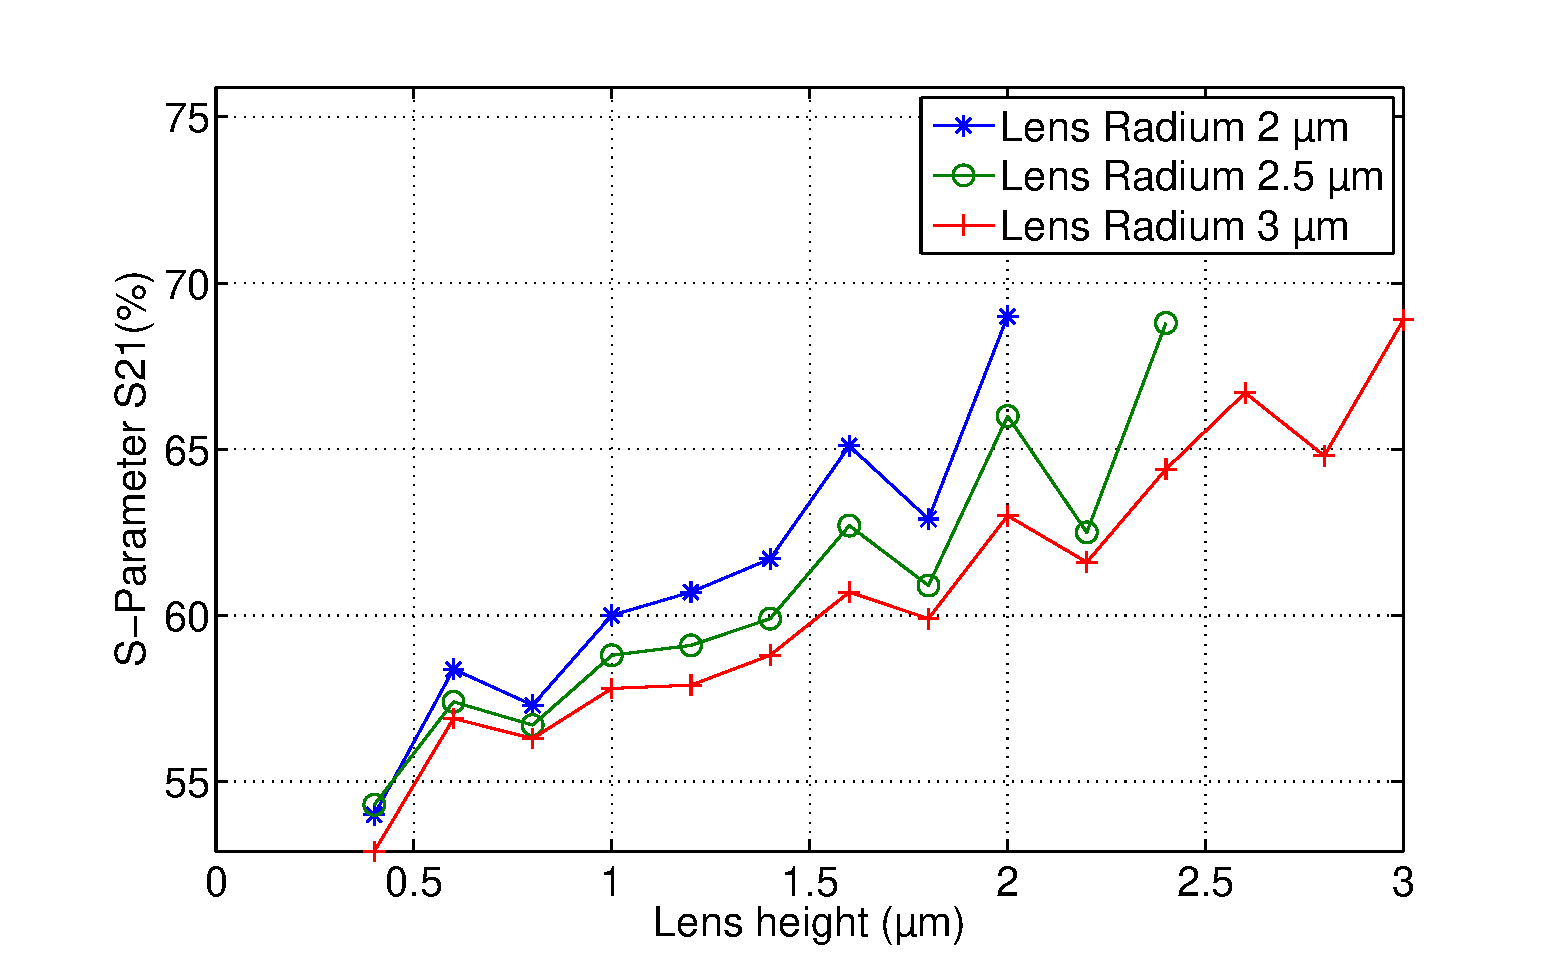
\includegraphics[width=0.8\textwidth]{bilder/s21_fix_lens_radium_hxx}
\caption{Coupling efficiency due to the variation of the lens height.}
\label{fig:coupling_lenses_curve_hxx}
\end{figure}

The reason of the efficiency change can be explained by Fig.  \ref{fig:matlab_coupling_lenses_rxx}-\ref{fig:matlab_coupling_lenses_rxx2}. From the former cure Fig. \ref{fig:matlab_coupling_lenses_rxx} we can tell that beam spot size at the working distance is bigger than the dimensions of the waveguide interface and from Fig. \ref{fig:matlab_coupling_lenses_rxx2} we understand the reason because rays near margin are penetrating mostly into substrate. In Fig. \ref{fig:matlab_coupling_lenses_rxx} rays near margin are refracted and focused to axis, so that the beam spot size is decreased and more rays are concentrated into waveguide to make the coupling become more adaptable.\\   
\begin{figure}[!ht]
\centering
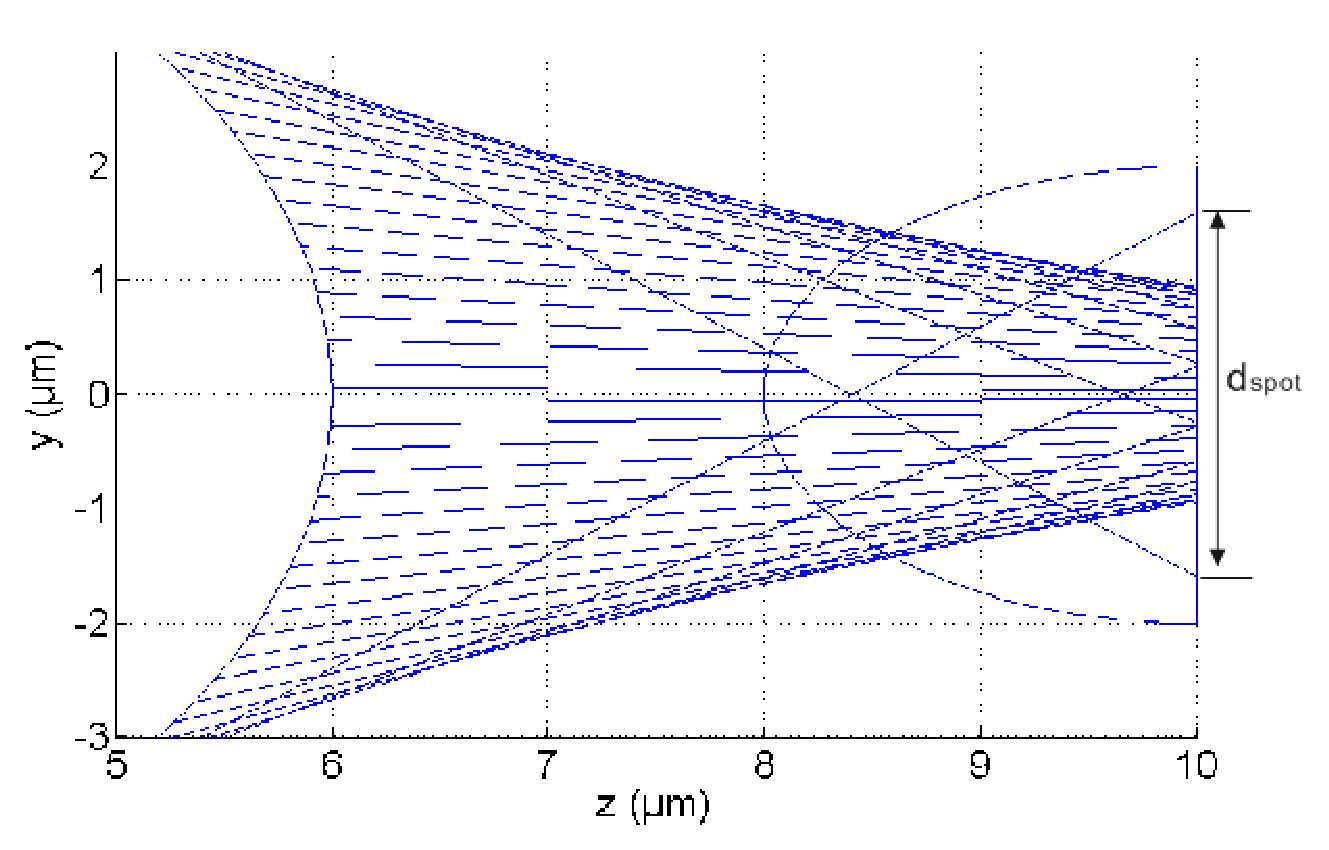
\includegraphics[width=0.8\textwidth]{bilder/beam_ray_without_refract}
\caption{The marginal rays propagate without refraction.}
\label{fig:matlab_coupling_lenses_rxx}
\end{figure}
\begin{figure}[!ht]
\centering
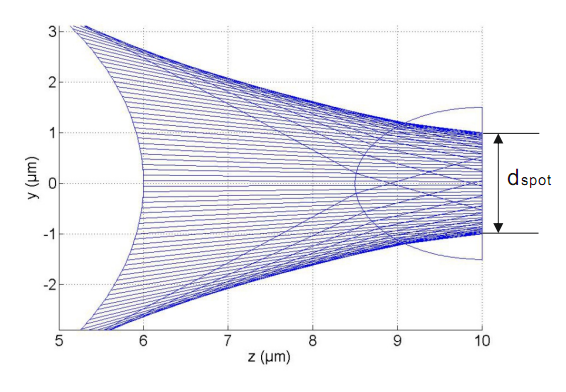
\includegraphics[width=0.8\textwidth]{bilder/beam_ray_refract}
\caption{The marginal rays are concentrated by lens of the waveguide.}
\label{fig:matlab_coupling_lenses_rxx2}
\end{figure}
For more information about the spot size of this configuration we can draw the Fig. \ref{fig:lensed_guide_spot_size_curve}. And the spot sizes changing agree well with the corresponding coupling efficiency.
\begin{figure}[!ht]
\centering
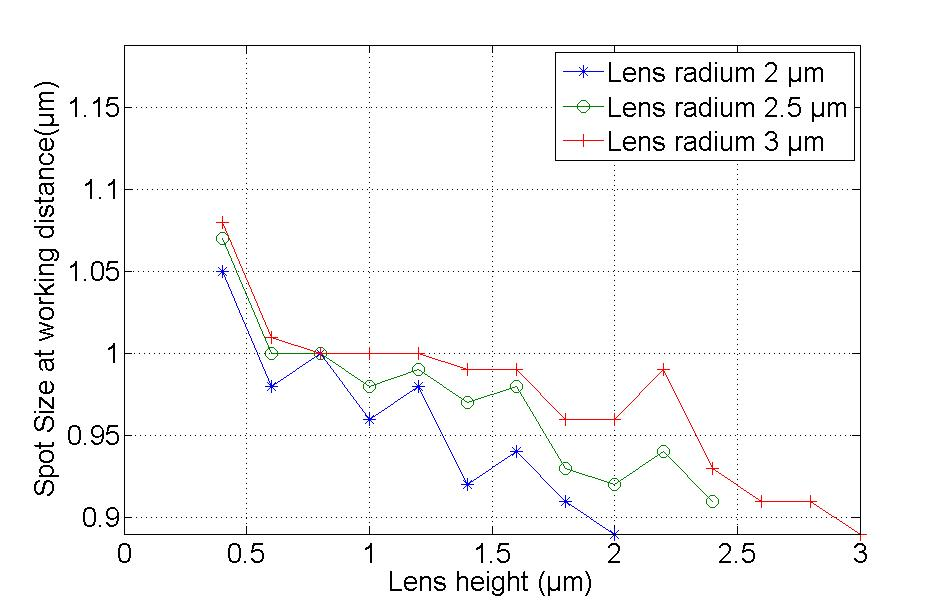
\includegraphics[width=0.8\textwidth]{bilder/spot_fix_lens_radium_hxx}
\caption{The spot size curve at lensed waveguide interface due to changing lens height}
\label{fig:lensed_guide_spot_size_curve}
\end{figure}
